\documentclass[border=3pt]{standalone}
\usepackage[T1]{fontenc}
\usepackage[utf8]{inputenc}
\usepackage{lmodern}
\usepackage{amsmath,amssymb}
\usepackage{xcolor}
\usepackage{tikz}
\usepackage{fontawesome5}
\usepackage{ragged2e}
\usetikzlibrary{shapes,shapes.geometric,shapes.misc,arrows.meta,positioning,
                calc,fit,backgrounds,decorations.pathreplacing,
                decorations.markings,patterns,chains}
\usetikzlibrary{decorations.pathreplacing,decorations.markings}
\definecolor{primary}{HTML}{1A5276}
\definecolor{secondary}{HTML}{2E86C1}
\definecolor{accent}{HTML}{E74C3C}
\definecolor{lightbg}{HTML}{EBF5FB}
\definecolor{defbg}{HTML}{FDF2E9}
\definecolor{greenhl}{HTML}{27AE60}
\definecolor{purplehl}{HTML}{8E44AD}
\definecolor{goldhl}{HTML}{B7950B}
\definecolor{tealhl}{HTML}{117A65}
\definecolor{codebg}{HTML}{F4F6F7}
\definecolor{neutral}{HTML}{707B7C}
\definecolor{dom1}{HTML}{1F618D}
\definecolor{dom2}{HTML}{117864}
\definecolor{dom3}{HTML}{6C3483}
\definecolor{dom4}{HTML}{922B21}
\definecolor{dom5}{HTML}{B7950B}
% --- carried over from ccna.sty so figures match the book exactly
\tikzset{
  dev/.style={rounded corners=3pt, draw=#1, fill=#1!8, text=#1!45!black,
              line width=0.9pt, minimum width=1.45cm, minimum height=1.05cm,
              align=center, font=\scriptsize\bfseries, inner sep=2pt},
  wirestyle/.style={line width=0.9pt, neutral!75},
  xconn/.style={line width=0.9pt, neutral!75, dash pattern=on 2.5pt off 2pt},
}

\newcommand{\Rtr}[3]{\node[dev=dom3] (#1) at #2 {\faIcon{route}\\#3};}
\newcommand{\Sw}[3]{\node[dev=dom2] (#1) at #2 {\faIcon{sitemap}\\#3};}
\newcommand{\Msw}[3]{\node[dev=dom3] (#1) at #2 {\faIcon{layer-group}\\#3};}
\newcommand{\Host}[3]{\node[dev=neutral] (#1) at #2 {\faIcon{desktop}\\#3};}
\newcommand{\Lap}[3]{\node[dev=neutral] (#1) at #2 {\faIcon{laptop}\\#3};}
\newcommand{\Srv}[3]{\node[dev=dom1] (#1) at #2 {\faIcon{server}\\#3};}
\newcommand{\Ap}[3]{\node[dev=dom5] (#1) at #2 {\faIcon{wifi}\\#3};}
\newcommand{\Wlc}[3]{\node[dev=dom5] (#1) at #2 {\faIcon{broadcast-tower}\\#3};}
\newcommand{\Fw}[3]{\node[dev=dom4] (#1) at #2 {\faIcon{shield-alt}\\#3};}
\newcommand{\Cld}[3]{\node[dev=neutral] (#1) at #2 {\faIcon{cloud}\\#3};}
\newcommand{\Phone}[3]{\node[dev=dom5] (#1) at #2 {\faIcon{phone-alt}\\#3};}
\newcommand{\Prn}[3]{\node[dev=neutral] (#1) at #2 {\faIcon{print}\\#3};}

% A link. The optional argument takes tikz options (e.g. xconn for a
% trunk drawn dashed); the fourth argument labels the link.
\newcommand{\wire}[4][wirestyle]{%
  \draw[#1] (#2) -- node[font=\tiny, text=neutral!85!black, fill=white,
                          inner sep=1.2pt, midway] {#4} (#3);}
\newcommand{\plainwire}[3][wirestyle]{\draw[#1] (#2) -- (#3);}


\newenvironment{topology}[1][]
  {\begin{center}\begin{tikzpicture}[font=\scriptsize,#1]}
  {\end{tikzpicture}\end{center}}


\newcommand{\cmd}[1]{\texttt{\small #1}}
\newcommand{\term}[1]{\textbf{\textcolor{primary}{#1}}}
\newcommand{\chref}[1]{Chapter~\ref{ch:#1}}
\newcommand{\ccnafitw}[1]{#1}
\providecommand{\thefigure}{}
% --- progressive builds
\newcount\buildlevel \buildlevel=99
% \stepvis{n}{..} appears from level n onward; \steponly{n}{..} at
% level n alone, which is how a caption is swapped rather than
% accumulated as the build advances. \stepdim{n}{..} is the
% complement of \stepvis: it shows only BEFORE level n, so a
% pair of them draws an element faint and then solid. That keeps
% the canvas full from step 1, which matters for a figure whose
% shape is itself the lesson -- a five-rung ladder revealed one
% rung at a time leaves a void where the method should be.
\newcommand{\stepvis}[2]{\ifnum#1>\buildlevel\relax\else#2\fi}
\newcommand{\steponly}[2]{\ifnum#1=\buildlevel #2\fi}
\newcommand{\stepdim}[2]{\ifnum#1>\buildlevel #2\fi}
% Slide text does not hyphenate. A projected caption broken as
% ``uni-cast'' costs the reader a beat that print can afford and a
% lecture cannot, and the ragged edge it avoids is invisible at
% four metres anyway.
\hyphenpenalty=10000 \exhyphenpenalty=10000
\begin{document}
\buildlevel=3
% Slide build of Figure 25.1 -- five defences, one at a time.
%
% Chapter 25 is the longest deck in the course, and this figure is what holds
% it together: five features that look like five unrelated commands until you
% see that all five hang off one untrusted port. Shown at once it is a wall of
% five boxes; built, each box arrives as the answer to "and what stops THIS?".
%
% The question leads the answer by one beat. Level n poses attack n and shows
% only the defences already named; level n+1 fills the slot. Putting both on
% the same beat -- which is what the obvious \stepvis{n}/\steponly{n} pairing
% does -- prints the answer beside the question and wastes it.
%
% Like the ladder, the shape is part of the lesson, so the five slots are drawn
% faint from the start: the room can see there are five, and "what are the
% other three?" is a better question to leave hanging than to spoil.
\begin{tikzpicture}[font=\scriptsize]
  \path (-1.1,-4.8) rectangle (14.4,1.3);

  \tikzset{
    dv/.style={rounded corners=3pt, draw=#1, fill=#1!8, text=#1!45!black,
               line width=0.9pt, minimum width=1.6cm, minimum height=1.0cm,
               align=center, font=\tiny\bfseries},
    ft/.style={rounded corners=3pt, draw=dom4!70, fill=dom4!7, line width=0.8pt,
               text width=2.5cm, align=center, font=\tiny,
               text=dom4!40!black, inner sep=4pt, minimum height=1.35cm},
    slot/.style={rounded corners=3pt, draw=neutral!25, fill=neutral!3,
                 line width=0.8pt, text width=2.5cm, align=center,
                 font=\tiny, text=neutral!35, inner sep=4pt,
                 minimum height=1.35cm},
    w/.style={line width=0.9pt, neutral!65},
    lk/.style={dom4!45, line width=0.7pt, dash pattern=on 2pt off 2pt},
    stepcap/.style={font=\bfseries, anchor=north west, text width=15.0cm,
                    align=left}}

  \node[dv=neutral] (h)  at (0,0)   {\faIcon{laptop}\\attacker\\or user};
  \node[dv=dom2, minimum width=2.0cm] (sw) at (5.0,0) {\faIcon{sitemap}\\SW1};
  \node[dv=dom3] (up) at (10.0,0) {\faIcon{route}\\uplink};
  \draw[w, line width=1.5pt] (h) -- (sw);
  \draw[w] (sw) -- (up);
  \node[font=\tiny\bfseries, text=accent!70!black] at (2.2,0.5)
      {untrusted access port};
  \node[font=\tiny\bfseries, text=dom2!45!black] at (7.5,0.5) {trusted uplink};

  % Empty slots for the defences not yet named. The number of them is the
  % point; their contents are the answer to a question worth asking first.
  \foreach \n/\x in {2/-0.6, 3/2.4, 4/5.4, 5/8.4, 6/11.4}
    {\stepdim{\n}{\node[slot, anchor=north west] at (\x,-1.5) {?};}}

  \stepvis{2}{\node[ft, anchor=north west] at (-0.6,-1.5)
      {\textbf{\faIcon{id-badge}~Port security}\\[2pt]stops many MACs, or the
       wrong one};}
  \stepvis{3}{\node[ft, anchor=north west] at (2.4,-1.5)
      {\textbf{\faIcon{address-card}~DHCP snooping}\\[2pt]stops a rogue DHCP
       server};}
  \stepvis{4}{\node[ft, anchor=north west] at (5.4,-1.5)
      {\textbf{\faIcon{exchange-alt}~Dynamic ARP inspection}\\[2pt]stops ARP
       poisoning};}
  \stepvis{5}{\node[ft, anchor=north west] at (8.4,-1.5)
      {\textbf{\faIcon{water}~Storm control}\\[2pt]stops flooding the
       segment};}
  \stepvis{6}{\node[ft, anchor=north west] at (11.4,-1.5)
      {\textbf{\faIcon{shield-alt}~RA guard}\\[2pt]stops a rogue IPv6
       router};}

  % The brace and the leader are structural, so they are present throughout:
  % they say "all of these hang off that one port" before any of them is named.
  \draw[lk, decorate, decoration={brace, amplitude=4pt, mirror}]
      (-0.6,-1.35) -- (13.9,-1.35);
  \draw[lk] (2.5,-0.35) -- (2.5,-1.25);

  \steponly{1}{\node[stepcap, text=dom4!45!black] at (-1.0,-3.3)
      {A host that sends thousands of source MACs fills the table and turns the
       switch into a hub. What stops it?};}
  \steponly{2}{\node[stepcap, text=dom4!45!black] at (-1.0,-3.3)
      {A laptop answering DHCP faster than the real server becomes the default
       gateway for the whole floor. What stops that?};}
  \steponly{3}{\node[stepcap, text=dom4!45!black] at (-1.0,-3.3)
      {A host that answers ARP for an address it does not own then reads
       everyone's traffic. What stops that?};}
  \steponly{4}{\node[stepcap, text=dom4!45!black] at (-1.0,-3.3)
      {A loop, or one broken NIC, floods the segment until nothing else gets
       through. What stops that?};}
  \steponly{5}{\node[stepcap, text=dom4!45!black] at (-1.0,-3.3)
      {IPv6 hosts pick their router from an advertisement that anyone on the
       segment can send. And that one?};}
  \steponly{6}{\node[stepcap, text=dom4!45!black] at (-1.0,-3.3)
      {Five features, five abuses, one port. All five live on the \emph{access}
       port, and all five exist because the device plugged into it is not under
       your control.};}
\end{tikzpicture}

\end{document}
